\chapter{Implementation}
\label{chap:implementation}

This chapter presents an in-depth description of how \f{} works
and demonstrates how much it can simplify developers' experience
by showing real-world examples with extensive usage of its features.
Furthermore, since we are creating an open-source project, the structure of
the repository will also be analyzed.


\section{Overview}

\f{} is a transpiler which enhances serverless programming by introducing the concept of annotations.
Annotations are an abstraction layer that the developers can unobtrusively use
to apply code transformations and metadata generation to a given application,
which will be deployed to a serverless platform.

To achieve this goal, we used the \textit{TypeScript}\cite{ts} compiler API which lets us
manipulate sources with ease, and \textit{SLS}\cite{sls} which
uses the generated metadata to deploy to \textit{AWS Lambda}.

\begin{figure}[H]
  \centering
  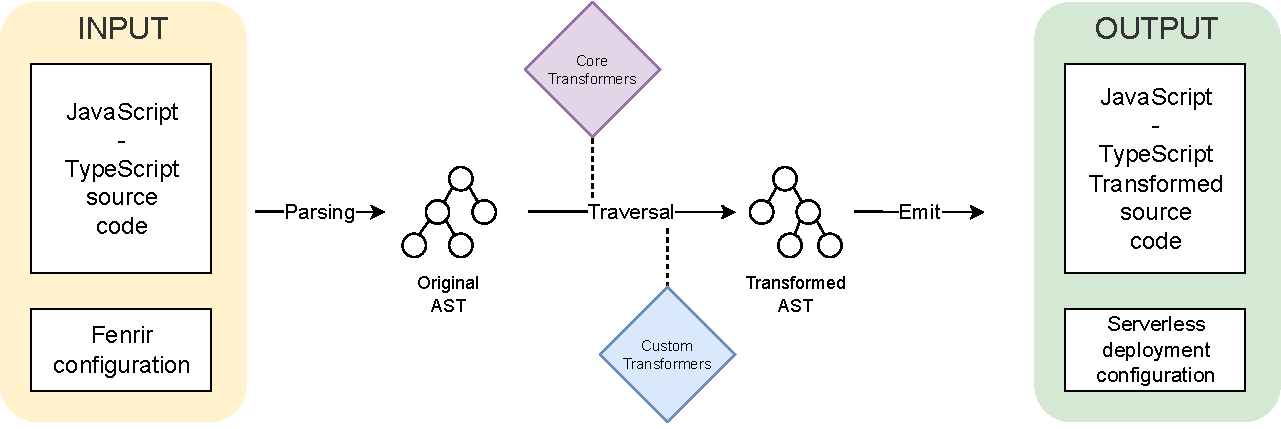
\includegraphics[width=\textwidth]{diagrams/pipeline}
  \caption{Transpiler pipeline.}
  \label{fig:pipeline}
\end{figure}

The transpilation pipeline, depicted in Figure \ref{fig:pipeline},
starts with the parsing of the input source code, which produces AST nodes with their related
annotations. Then, each annotation induces the application of its related
transformation step, whose output is fed into the next transformer, if any.
During the transformation steps, \f{} reports possible errors by gracefully
stopping the compilation process and indicating the offending instructions. Once
the transformations have taken place without any errors, the output code is saved
and the related metadata is also appended to a
\verb|serverless.yml| file which specifies function deployment
properties (e.g., the address to invoke a given function).

It is important to notice that \f{} doesn't lock developers in managing their
functions only through its tools, instead, its primary objective is to facilitate
the incremental adoption of the serverless paradigm.

\subsection{Brief example: Monolith to Serverless conversion}

Lorem ipsum dolor sit amet, qui minim labore adipisicing minim sint cillum sint consectetur cupidatat.

% \section{Detailed review}

% This section explains each step of the pipeline, defines annotations precisely and shows how to create new ones.

\section{Parsing}

\f{} requires a configuration file that must be named \verb|fenrir.config.json| to understand where to operate:

\begin{lstlisting}[language=json]
{
  "files": ["input/source.ts"],
  "serverlessConfigPath": "input/serverless.yml",
  "outputDirectory": "output",
  "annotations": {
    "CustomAnnotation": "annotations/custom-annotation.ts"
  }
}
\end{lstlisting}

The \verb|files| field accepts an array of filenames or a directory,
and it is used to represent which files will be parsed by the transpiler.

The \verb|serverlessConfigPath| field points at the input \textit{SLS} configuration
that must contain some mandatory input metadata, such as the region which the functions will be deployed on.

The \verb|outputDirectory| field indicates where the emitted files will be placed.

The \verb|annotations| field locates custom annotations as it takes an object
where the keys represent the new names and the values refer to their associated implementations.

\paragraph{\textbf{Fenrir's CLI}}
After creating the configuration, \f{} can be started through our CLI tool
by optionally passing as a flag the directory in which it is contained.
\begin{lstlisting}[language=bash, style=bashstyle]
# defaults to the current directory (.) for its file lookup...
> fenrir
# ...or uses a custom path
> fenrir -g input-directory
\end{lstlisting}
Furthermore, the CLI offers the \verb|init| sub-command to ease the setup needed for the entire pipeline
by generating the necessary boilerplate and configuration files.

% TODO: ricorda di parlare di quanto sia ottimo il compiler api di ts in Background.
% perché ha informazioni su tutto il progetto e non solo sui file.
\subsubsection{AST Traversal}

Through the \textit{TypeScript} compiler API, each sources' AST is traversed
by a visitor function which collects some data (e.g., dependencies imports) and examines
certain types of node in order to process annotations, namely \textit{exported function declarations}.
Lookups are restricted only to this syntactic category for two reasons:
\begin{itemize}
  \item \verb|export| ensures the functions are public and ready to be deployed.
  \item \verb|function declarations| minimize the code needed to control the AST.
    Considering that \textit{JavaScript} provides three distinct ways of declaring a function,
    accommodating all of these variations would inevitably result in a threefold expansion of the manipulation code.
    Moreover, function declarations are the idiomatic technique to write top-level functions.
\end{itemize}

\begin{lstlisting}[language=javascript, caption={Examples of processed or skipped nodes.}]
// Skipped
const a = 2;
// Skipped
for (const b of [1, 2, 3]) {}
// Processed
export function foo() {}
// Skipped
export const fiz = () => {}
// Skipped
export const bar = function() {}
\end{lstlisting}

The processed functions have their annotations examined, and
their bodies are visited to handle AST transformations.

\section{Annotations}

Annotations are syntactical units, or keywords, enclosed within JSDoc comments,
each associated with their respective transformer.
They can be expressed using a BNF-like syntax:
\begin{equation*}
\begin{aligned}
    \text{Annotation} & ::= "\$" \langle \text{Name} \rangle [ "(" \langle \text{Parameters} \rangle ")" ] \\
    \text{Name} & ::= [\text{a-zA-Z\_}][\text{a-zA-Z0-9\_}]* \\
    \text{Parameters} & ::= \langle \text{TypeScriptObject} \rangle \\
    \text{TypeScriptObject} & ::= \dots \\
\end{aligned}
\end{equation*}
This representation does not intend to provide a formal and precise depiction of the syntax of annotations.
Nevertheless, it serves to offer a general impression of how they can be written within the code.
\begin{lstlisting}[language=javascript, caption={Generic examples of annotation.}, label={lst:annotations-examples}]
/** $\dollar$Foo */

/** $\dollar$Bar(param: "first") */

/** $\dollar$Fiz(first: true, second: [1, 2, 3], third: (a, b) => a + b) */

/**
 * Annotations enrich docs...
 * $\dollar$Foo
 * ...and can even be multiline.
 * $\dollar$Bar(
 *    param: "fiz"
 * )
 *
 * all these explanatory texts are not 
 * harmful, as they are simply ignored.
 */
\end{lstlisting}

Annotations are designed to avoid cluttering \textit{JavaScript} with new syntax,
as they can only be written inside JSDoc comments.
Thus, they serve a dual-purpose by not only providing functionality
but also serving as supplementary documentation for the codebase.

Listing \ref{lst:annotations-examples} provides a valuable insight on how annotations
may be parameterized to modify transformers' functionality.
In fact, arguments undergo parsing as a \textit{TypeScript} object literal,
hence, they are as powerful as regular objects\cite{mdn_objects}
meaning that even complex structures (arrays, functions, etc...) can be used
during the compilation step to enrich transformations.

Another crucial feature of annotations is their composability,
as multiple annotations can be written within the same JSDoc,
essentially defining dedicated compilation pipelines by passing the output
of a transformation as input for the subsequent ones:
to facilitate this process, each source file may be visited multiple times.

\subsection{Core Annotations}

\f{} offers four core annotations whose transformers can handle code manipulation,
deployment metadata, or a combination of both functionalities:
by pipelining annotations, we can effectively utilize the strengths of different approaches.

\begin{table}[htbp]
    \centering
    \caption{Core annotations}
    \begin{tabular}{llcc}
        \toprule
        \textbf{Name} & \textbf{Code} & \textbf{Metadata} \\
        \midrule
        \$Fixed & Yes & Yes \\
        \$TrackMetrics & Yes & No \\
        \$HttpApi & No & Yes \\
        \$Scheduled & No & Yes \\
        \bottomrule
    \end{tabular}
\end{table}

\subsubsection{\$Fixed}
\annotation{\$Fixed(memorySize?: number, timeout?: number, ...)}
converts monolithic functions into \textbf{fixed}-size serverless functions,
whose resources are statically determined and remain constant regardless of the workload or input size.
To achieve this conversion, code is handled as follows:
\begin{itemize}
  \item The monolithic functions' parameters are mapped to a single \verb|event|
    parameter in order to adhere to \textit{AWS Lambda} serverless functions' signature.
  \item The monolithic functions' return statements change to match
    the shape of the response expected by the platform,
    by creating an object with a status code (\verb|200|)
    and a body that contains a serialized version of the initially returned value.
  \item Early return statements and throw statements are modified similarly,
    but the status code represents a client error (\verb|400|).
\end{itemize}

\annotation{\$Fixed} has no mandatory parameters, however, all the specified arguments will be
passed as metadata for the function deployment.

% ----------------------------------------------------------
% FIXED EXAMPLE
% ----------------------------------------------------------

\begin{lstlisting}[language=javascript, caption={Input code}]
/** $\dollar$Fixed(timeout: 10) */
export async function foo(id) {
  if (!isValid(id)) {
    throw new Error('Something went wrong')
  }

  const data = await query()

  return data
}
\end{lstlisting}


\begin{lstlisting}[language=javascript, caption={Output code}]
/** $\dollar$Fixed(timeout: 10) */
export async function foo(event) {
  const id = event.id

  if (!isValid(id)) {
    return {
      statusCode: 400,
      body: JSON.stringify({
        error: "'Something went wrong'",
      }),
    }
  }

  const data = await query()

  return {
    statusCode: 200,
    body: JSON.stringify(data),
  }
}
\end{lstlisting}

\begin{lstlisting}[language=yaml, caption={Generated Metadata through \annotation{$\dollar$Fixed}}]
# Generated metadata
functions:
  foo:
    handler: output/source.foo
  timeout: 10 # default is 6 seconds
\end{lstlisting}
% ----------------------------------------------------------
% FIXED EXAMPLE
% ----------------------------------------------------------

\subsection{Custom Annotations}

Lorem ipsum dolor sit amet, qui minim labore adipisicing minim sint cillum sint consectetur cupidatat.

\section{Emit}

Magari parlare della gestione degli errori. E poi dell'emit.
E di come gli argomenti sono trattati.
